
\documentclass{article}
\usepackage[headheight=20pt, margin=1.0in, top=1.2in]{geometry}
\usepackage{amsmath, amssymb, amsthm, thmtools, tcolorbox, array, graphicx, makeidx, cancel, multirow, fancyhdr, xypic, color, nicefrac, rotating, multicol, caption, subcaption, xcolor, tikz, tikz-3dplot, tikz-cd, pgfplots, import, enumitem, calc, booktabs, wrapfig, siunitx, hyperref,float}
\hypersetup{colorlinks=true,linkcolor=blue}
\usepackage[all]{xy}
\usepackage{esint}
\setlength{\parindent}{0in}
\sisetup{per-mode = symbol}
\usetikzlibrary{calc,arrows,svg.path,decorations.markings,patterns,matrix,3d,fit}
\usepgfplotslibrary{groupplots}
\pgfplotsset{compat=newest}
\newtcolorbox{mydefbox}[2][]{colback=red!5!white,colframe=red!75!black,fonttitle=\bfseries,title=#2,#1}
\newtcolorbox{mythmbox}[2][]{colback=gray!5!white,colframe=gray!75!black,fonttitle=\bfseries,title=#2,#1}
\newtcolorbox{myexamplebox}[2][]{colback=green!5!white,colframe=green!75!black,fonttitle=\bfseries,title=#2,#1}
\newtcolorbox{mypropbox}[2][]{colback=blue!5!white,colframe=blue!75!black,fonttitle=\bfseries,title=#2,#1}
\declaretheoremstyle[headfont=\color{blue}\normalfont\bfseries,]{colored}
\theoremstyle{definition}
\newtheorem{theorem}{Theorem}
\newtheorem{corollary}[theorem]{Corollary}
\newtheorem{lemma}[theorem]{Lemma}
\newtheorem{proposition}[theorem]{Proposition}
\newtheorem{problem}[theorem]{Problem}
\newtheorem{definition}[theorem]{Definition}
\newtheorem{exercise}[theorem]{Exercise}
\newtheorem{example}[theorem]{Example}
\newtheorem{solution}[theorem]{Solution}
\newtheorem*{thm}{Theorem}
\newtheorem*{lem}{Lemma}
\newtheorem*{prob}{Problem}
\newtheorem*{exer}{Exercise}
\newtheorem*{prop}{Proposition}
\def\R{\mathbb{R}}
\def\F{\mathbb{F}}
\def\Q{\mathbb{Q}}
\def\C{\mathbb{C}}
\def\N{\mathbb{N}}
\def\Z{\mathbb{Z}}
\def\Ra{\Rightarrow}
\def\e{\epsilon}
\newcommand{\typo}[1]{{\color{red}{#1}}}
\newcommand\thedate{\today}
\newcommand{\mb}{\textbf}
\newcommand{\norm}[2]{\|{#1}\|_{#2}}
\newcommand{\normm}[1]{\|#1\|}
\newcommand{\mat}[1]{\begin{bmatrix} #1 \end{bmatrix}}
\newcommand{\eqtext}[1]{\hspace{3mm} \text{#1} \hspace{3mm}}
\newcommand{\set}[1]{\{#1\}}
\newcommand{\inte}{\textrm{int}}
\newcommand{\ra}{\rightarrow}
\newcommand{\minv}{^{-1}}
\newcommand{\tx}[1]{\text{ {#1} }}
\newcommand{\abs}[1]{|#1|}
\newcommand{\mc}[1]{\mathcal{#1}}
\newcommand{\uniflim}{\mathop{\mathrm{unif\lim}}}
\newcommand{\notimplies}{\mathrel{{\ooalign{\hidewidth$\not\phantom{=}$\hidewidth\cr$\implies$}}}}
\pagestyle{fancy}
\fancyhf{}
\fancyhead[L]{Title of the Document}
\fancyhead[C]{}
\fancyhead[R]{\thepage}
\fancyfoot[L]{}
\fancyfoot[C]{}
\fancyfoot[R]{}
\renewcommand{\headrulewidth}{0.4pt}
\renewcommand{\footrulewidth}{0.4pt}
\numberwithin{equation}{section}
% Increase spacing between paragraphs
\setlength{\parskip}{1em}
% Increase spacing before and after sections
\usepackage{titlesec}
\titlespacing*{\section}{0pt}{3ex plus 1ex minus .2ex}{2ex plus .2ex}
\titlespacing*{\subsection}{0pt}{2ex plus 1ex minus .2ex}{1ex plus .2ex}
\titlespacing*{\subsubsection}{0pt}{1ex plus 1ex minus .2ex}{1ex plus .2ex}
\title{\textbf{Title of the Document}}
\author{Author Name}
\date{\today}
\begin{document}
\maketitle
\tableofcontents
\newpage
\section{Interior and Boundary Points}

\begin{mydefbox}
\textbf{Definition 2.1}

Let $(X,d)$ be a metric space. If $x \in X$ and $r > 0$, we define the \emph{open ball of radius} $r$ \emph{centered at} $x$ as 
$
    B_r(x) := \{y \in X : d(x,y) < r\}.
$
\end{mydefbox}

In $\mathbb{R}^n$ with the Euclidean metric $d(x,y) = \|x - y\|$, the open ball $B_r(x)$ is nothing more than the collection of points which are a distance at most $r$ from $x$. This generalizes the interval, since in $\mathbb{R}^1$ we have 
$
    B_r(x) = \{y \in \mathbb{R} : |x - y| < r\} = (x - r, x + r),
$
or if we centre around $0$, $B_r(0) = (-r, r)$. In $\mathbb{R}^2$ we get a disk of radius $r$, 
$
    B_r(0) = \{(x, y) \in \mathbb{R}^2 : \sqrt{x^2 + y^2} < r\},
$
which we recognize as being the same as $x^2 + y^2 < r^2$. 

\begin{center}
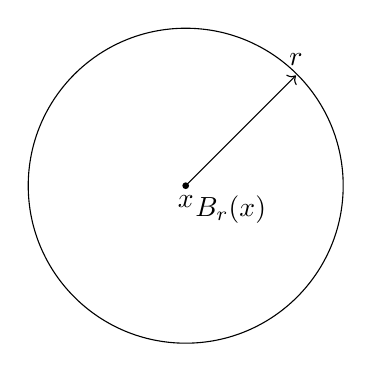
\begin{tikzpicture}
    \draw (0,0) circle (2) node[below right] {$B_r(x)$};
    \filldraw (0,0) node[below] {$x$} circle (1pt);
    \draw[->] (0,0) -- (1.4,1.4) node[above] {$r$};
\end{tikzpicture}

Figure 2.1: In $\mathbb{R}^2$, the open ball of radius $r$ centered at $x$ consists of all points which are a distance at most $r$ from $x$.
\end{center}

\begin{mydefbox}
\textbf{Definition 2.2}

A subspace $S$ of a metric space $X$ is \emph{bounded} if there exists an $r > 0$ and an $a \in X$ such that $S \subseteq B_r(a)$.
\end{mydefbox}

\begin{mydefbox}
\textbf{Definition 2.3}

Let $(X,d)$ be a metric space, and $S \subseteq \mathbb{R}^n$ be an arbitrary set. 

\begin{enumerate}
    \item We say that $x \in S$ is an \emph{interior point} of $S$ if there exists an $r > 0$ such that $B_r(x) \subseteq S$; that is, $x$ is an interior point if we can enclose it in an open ball which is entirely contained in $S$.
    \item We say that $x \in S$ is a \emph{boundary point} of $S$ if for every $r > 0$, $B_r(x) \cap S \neq \emptyset$ and $B_r(x) \cap \partial S \neq \emptyset$; that is, $x$ is a boundary point if no matter what ball we place around $x$, that ball lives both inside and outside of $S$.
\end{enumerate}
\end{mydefbox}

The \emph{interior of $S$} -- denoted $S^{\circ}$ -- is the collection of interior points of $S$, while \emph{boundary of $S$} -- denoted $\partial S$ -- is the collection of boundary points of $S$.

\begin{center}
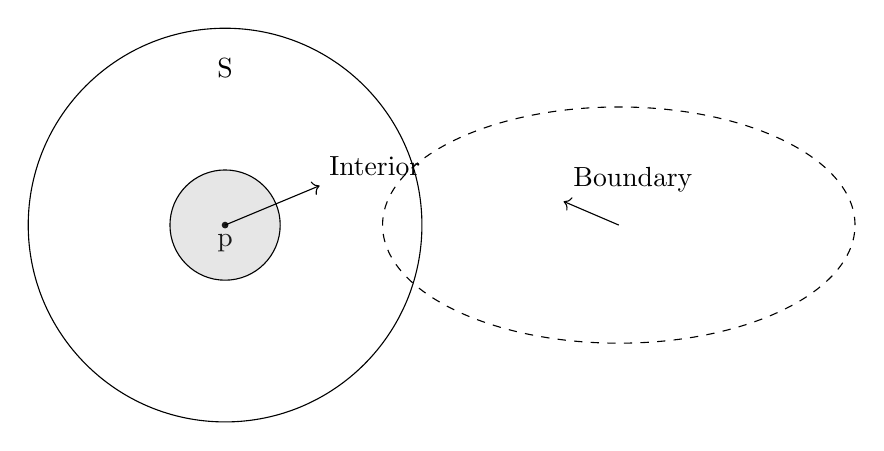
\begin{tikzpicture}
    \draw (2,2) circle (2.5);
    \draw[dashed] (7,2) ellipse (3 and 1.5);
    \node at (2, 4) {S};
    \filldraw (2, 2) circle (1pt) node[below] {p};
    \begin{scope}
        \clip (2, 2) circle (2.5);
        \draw[fill=gray, fill opacity=0.2] (2, 2) circle (0.7);
    \end{scope}
    \draw[->] (7,2) -- (6.3, 2.3) node[above right] {Boundary};
    \draw[->] (2,2) -- (3.2, 2.5) node[above right] {Interior};
\end{tikzpicture}

Figure 2.2: The point $b$ is a boundary point. No matter what size ball we place around $b$, that ball will intersect both $S$ and $\partial S$. On the other hand, $p$ is an interior point, since we can place a ball around it which lives entirely within $S$. 
\end{center}

We should take a moment and think about these definitions, and why they make sense. A boundary point is any point $x$ which occurs at the very fringe of the set; that is, if I push a little further I will leave the set. An interior point should be a point inside of $S$, such that if I move in any direction a sufficiently small distance, I stay within the set. Note that if $x$ is an interior point then we must have that $x \in S$; however, boundary points do \emph{not} need to be in the set. We start with a simple example.

\begin{myexamplebox}
 \textbf{Example 2.4} \\
 Let $S = (-1,1) \subseteq \mathbb{R}$ endowed with the Euclidean metric. What are the interior points and the boundary points of $S$? \\
 \end{myexamplebox}
 \textbf{Solution.} I claim that any point in $(-1,1)$ is an interior point. To see that this is the case, let $p \in (-1,1)$ be an arbitrary point. We need to place a ball around $p$ which lies entirely within $(-1,1)$. To do this, assume without loss of generality that $p \ge 0$. If $p = 0$ then we can set $r = 1/2$ and $B_r(p) \subseteq (-1/2,1/2) \subseteq (-1,1)$. Thus assume that $p \neq 0$ and let $r = (1-p)/2$, which represents half the distance from $p$ to 1. I claim that $B_r(p) \subseteq (-1,1)$. Indeed, let $x \in B_r(p)$ be any point, so that $|x-p| < r$ by definition. Then 
 $
 |x| = |x - p + p| \leq |x - p| + p \\
 \leq r + p = \frac{1 - p}{2} + p \\
 = \frac{1 + p}{2} < 1
 $
where in the last inequality we have used the fact that $p < 1$ so $1 + p < 2$. Thus $x \in (-1,1)$, and since $x$ was arbitrary, $B_r(p) \subseteq (-1,1)$.

The boundary points are $\pm1$, where we note that even though $-1 \notin (-1,1)$, it is still a boundary point. To see that $-1$ is a boundary point, let $r > 0$ be arbitrary, so that $B_r(p) = (-1-r,1+r)$. We then have 
$ 
B_r(p) \cap (-1,1) = (1 - r, 1) \neq \varnothing, \quad B_r(p) \cap (-1,1)^c = (1,1 + r) \neq \varnothing 
 $ 
as required. The proof for $-1$ is analogous and left as an exercise.

\begin{myexamplebox}
\textbf{Example 2.5} \\
What is the boundary of $\mathbb{Q}$ in $\mathbb{R}$ with the Euclidean metric?\\
\end{myexamplebox}
\textbf{Solution.} We claim that $\partial \mathbb{Q} = \mathbb{R}$. Since both the irrationals and rationals are dense in the real numbers, we know that every non-empty open interval in $\mathbb{R}$ contains both a rational and irrational number. Thus let $x \in \mathbb{R}$ be any real number, and $r > 0$ be arbitrary. The set $B_r(x)$ is an open interval around $x$, and contains a rational number, showing that $B_r(x) \cap \mathbb{Q} \neq \varnothing$. Similarly, $B_r(x)$ contains an irrational number demonstrating that $B_r(x) \cap \mathbb{Q}^c \neq \varnothing$, so $x \in \partial \mathbb{Q}$. Since $x$ was arbitrary, we conclude that $\partial \mathbb{Q} = \mathbb{R}$.

\section{Open and Closed Sets}

\begin{mydefbox}
\textbf{Definition 2.6} 

A set $S$ in a metric space $(X, d)$ is said to be open if every point of $S$ is an interior point; that is, $S$ is open if for every $x \in S$ there exists an $r > 0$ such that $D_{d}(x) \subseteq S$. The set $S$ is closed if $S^c$ is open. Given a point $x \in X$, an open nei {gh}borhood of $x$ is some open set containing $x$.
\end{mydefbox}

\begin{myexamplebox}
\textbf{Example 2.7}

The set $S=\{(x,y)\in\mathbb{R}^2 : y > 0\} \subset \mathbb{R}^2$ is open in the Euclidean metric.
\end{myexamplebox}

\section{Open, Closed, and Everything in Between}

\begin{center}
 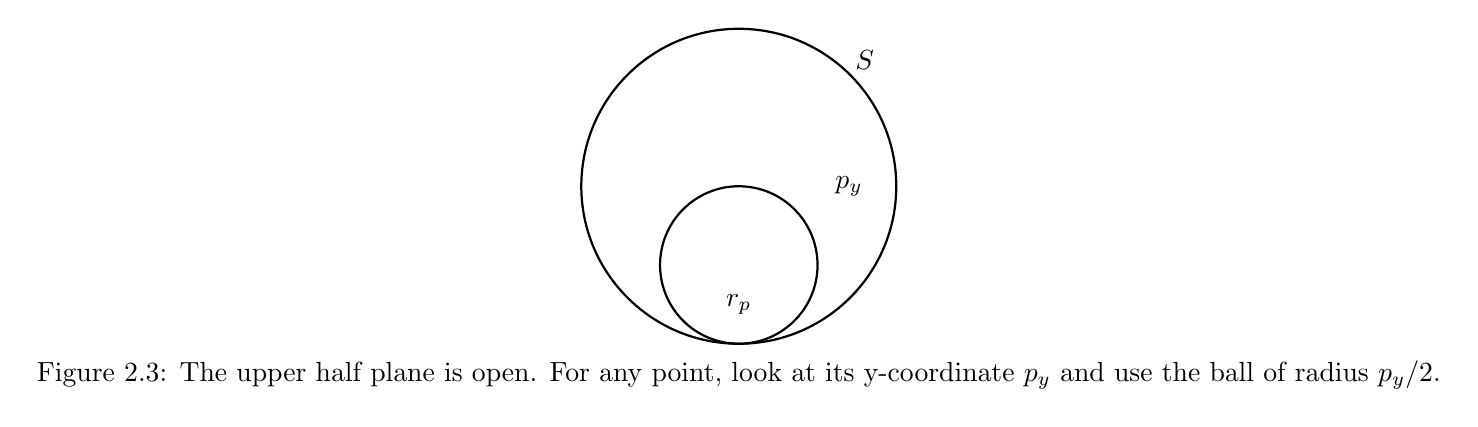
\begin{tikzpicture}
    \draw[thick] (0,0) circle (2);
    \node at (1.6,1.6) {$S$};
    \node at (0,-2.4) {Figure 2.3: The upper half plane is open. For any point, look at its y-coordinate $p_{y}$ and use the ball of radius $p_{y}/2$.};
    \draw[thick] (0,-1) circle (1);
    \node at (0,-1.5) {$r_{p}$};
    \node at (1.4, 0) {$p_{y}$};
\end{tikzpicture}
\end{center}

\begin{proof}
We need to show that around every point in $S$ we can place an open ball that remains entirely within $S$. Choose a point $p = (p_{x}, p_{y}) \in S$, so that $p_{y} > 0$, and let $r = p_{y}/2$. Consider the ball $B_{r}(p)$, which we claim lies entirely within $S$. To see that this is the case, choose any other point $q = (q_{x}, q_{y}) \in B_{r}(p)$. Now

$
|p_{y} - q_{y}| \leq \|q - p\| < r = \frac{p_{y}}{2}
$

which implies that $q_{y} > p_{y} - p_{y}/2 = p_{y}/2 > 0$. Since $q_{y} > 0$ this shows that $q \in S$, and since q was arbitrary, $B_{r}(p) \subseteq S$ as required. $\blacksquare$
\end{proof}\end{document}